\documentclass[tikz,border=10pt]{standalone}
\usetikzlibrary{calc}
\begin{document}
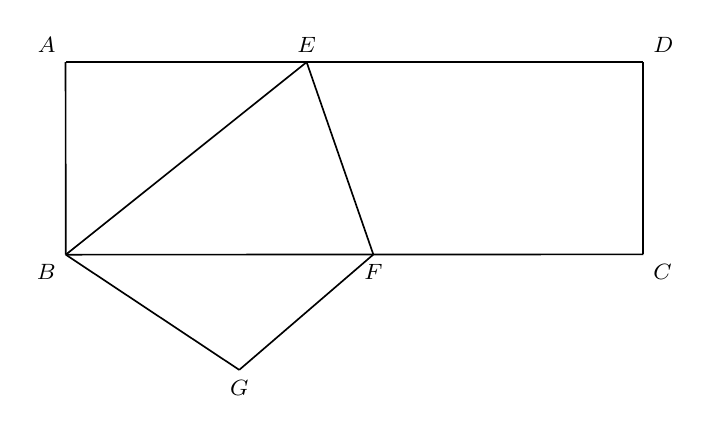
\begin{tikzpicture}[line width=0.6pt, line join=round]
\coordinate (A) at (-3.679,1.966);
\coordinate (B) at (-3.676,-0.480);
\coordinate (C) at (3.658,-0.476);
\coordinate (D) at (3.658,1.966);
\coordinate (F) at (0.230,-0.478);
\coordinate (G) at (-1.473,-1.943);



\coordinate (E) at (-0.617,1.965);


\draw (A) -- (D);
\draw (D) -- (C);
\draw (C) -- (B);
\draw (B) -- (A);


\draw (E) -- (B);
\draw (B) -- (G);
\draw (G) -- (F);
\draw (F) -- (E);




\node[above left]  at (A) {\fontsize{8}{9.6}\selectfont $A$};
\node[above right] at (D) {\fontsize{8}{9.6}\selectfont $D$};
\node[below right] at (C) {\fontsize{8}{9.6}\selectfont $C$};
\node[below left]  at (B) {\fontsize{8}{9.6}\selectfont $B$};
\node[above]       at (E) {\fontsize{8}{9.6}\selectfont $E$};
\node[below]       at (F) {\fontsize{8}{9.6}\selectfont $F$};
\node[below]       at (G) {\fontsize{8}{9.6}\selectfont $G$};
\end{tikzpicture}
\end{document}